\chapter{Конструкторская часть}

В данном разделе будут представлены требования к программному обеспечению, а также схемы алгоритмов, выбранных для решения задачи.

\section{Разработка алгоритмов}
В данном разделе будут представлены схемы реализации выбранных алгоритмов. 
\subsection{Общий алгоритм программы}
\begin{enumerate}
	\item Задать объекты сцены (интерьер комнаты, расположение источников света, характеристики источников дыма).
	\item Задать параметры частиц дыма.
	\item Запустить симуляцию.
	\item Отобразить полученное изображение.
\end{enumerate}

\subsection{Система частиц для реализации дыма}

На рисунке \ref{fig:particlemovesystem} показана схема алгоритма реализации движения частицы.

\begin{figure}[H]
	\centering
	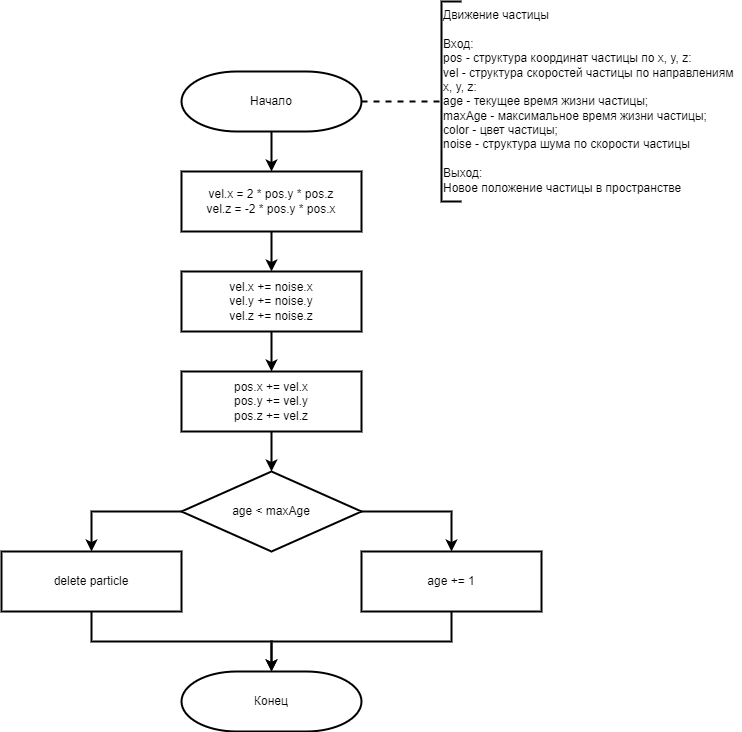
\includegraphics[width=1\linewidth]{inc/img/particle_move}
	\caption[]{Схема алгоритма системы движения частиц}
	\label{fig:particlemovesystem}
\end{figure}



\subsection{Алгоритм обратной трассировки лучей}

На рисунке \ref{fig:follow} представлена схема алгоритма обратной трассировки лучей.
\begin{figure}[H]
	\centering
	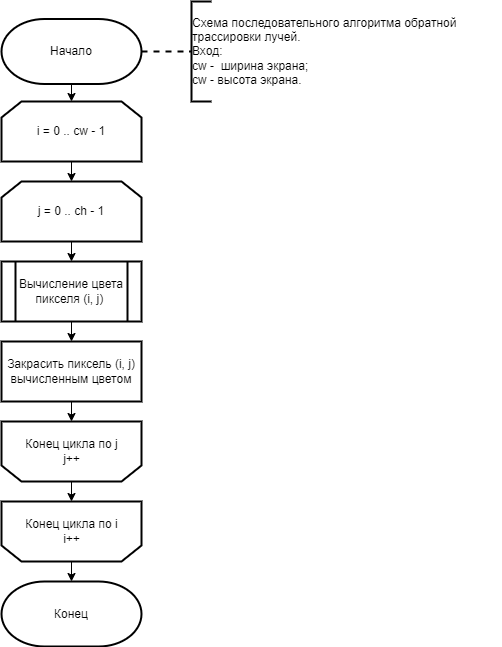
\includegraphics[width=0.7\linewidth]{inc/img/follow}
	\caption{Схема алгоритма обратной трассировки лучей}
	\label{fig:follow}
\end{figure}
\newpage
\section{Структура классов}
Классы в программе можно условно разделить на несколько групп по выполняемым функциям.

\begin{enumerate}
	\item Математические абстракции.
	\begin{itemize}[label=---]
		\item Ray - трехмерный луч, задающийся точкой начала луча, направляющим вектором;
		\item Point – радиус-вектор точки сцены.
	\end{itemize}
	\item Трехмерные объекты.
	\begin{itemize}[label=---]
		\item Model – класс хранящий в себе статический декоративный объект;
		\item Light – класс источника света, содержащий информацию о положении и интенсивности;
		\item Smoker – класс источника дыма, содержащий информацию о скорости генерации частиц и положении.
		\item Particle – класс частицы дыма, содержащий информацию о положении, скорости, времени жизни, размерах, цвете частицы.
	\end{itemize}
	\item Scene - характеризует набор объектов и их свойств.
	\item Интерфейс пользователя. Взаимодействие с интерфейсом происходит через диалоговые окна, которые в свою очередь взаимодействуют с классом Scene.
\end{enumerate}
\newpage
\section{Диаграмма классов}
На рисунке \ref{fig:classdiagramm} представлена диаграмма классов
\begin{figure}[H]
	\centering
	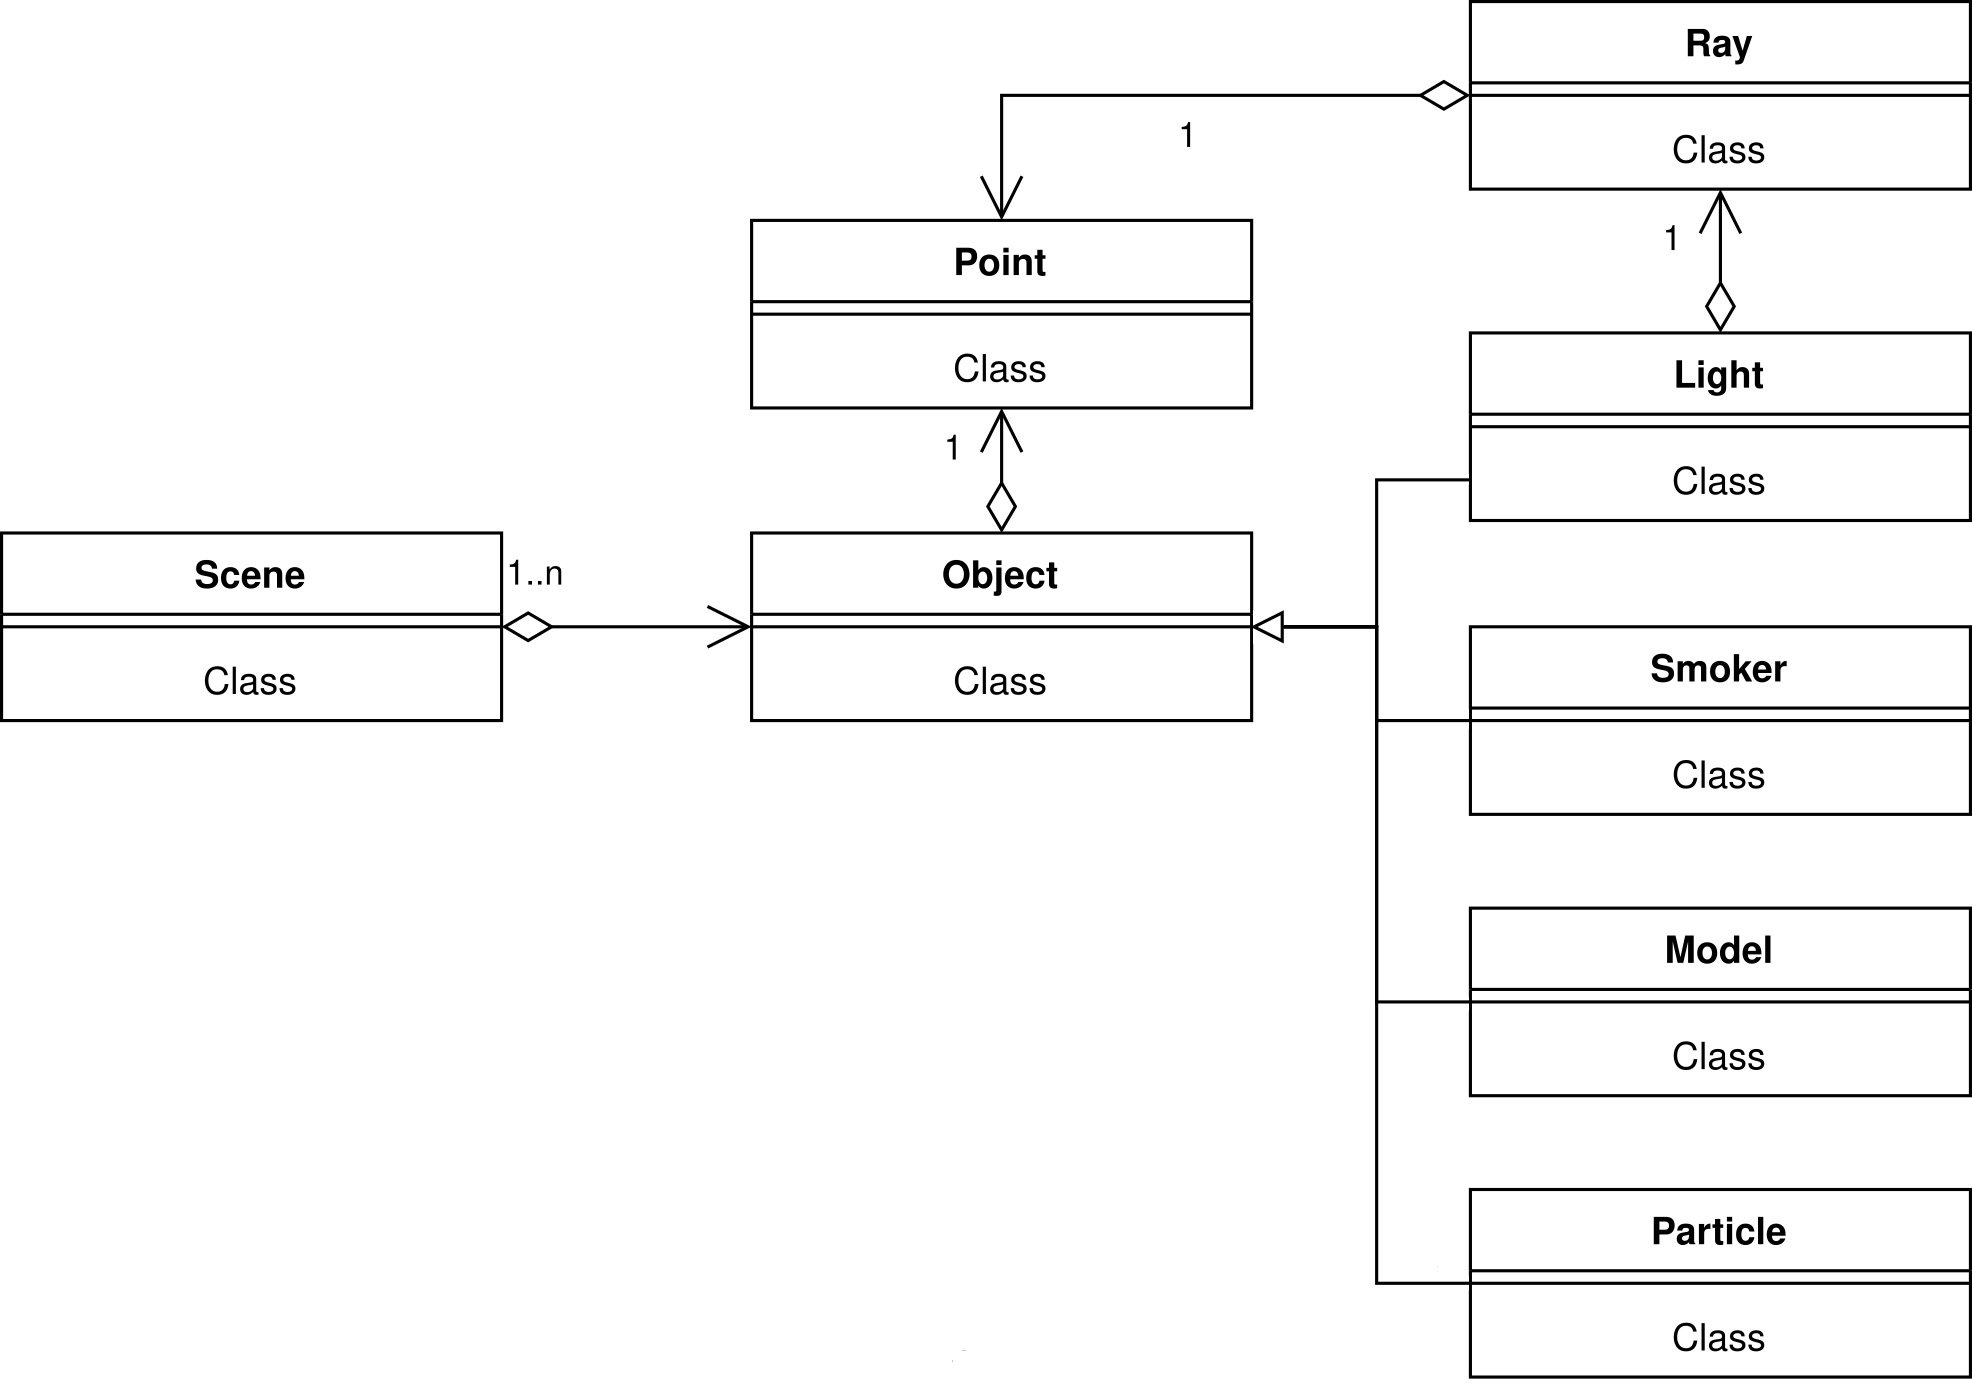
\includegraphics[width=1\linewidth]{inc/img/ClassDiagramm}
	\caption{Диаграмма классов}
	\label{fig:classdiagramm}
\end{figure}

\section*{Вывод}

В данном разделе были рассмотрены требования, которые выдвигаются программному продукту, схемы алгоритмов, а также типы и структуры данных, которые были использованы при реализации программного обеспечения.





